\chapter{圖論緣起}

\section{話說1736年}
\section{圖的定義}

\source{p.010}

\source{p.011}
關於 Ulam猜想的難點在於，如果有兩個圖：

\begin{center}
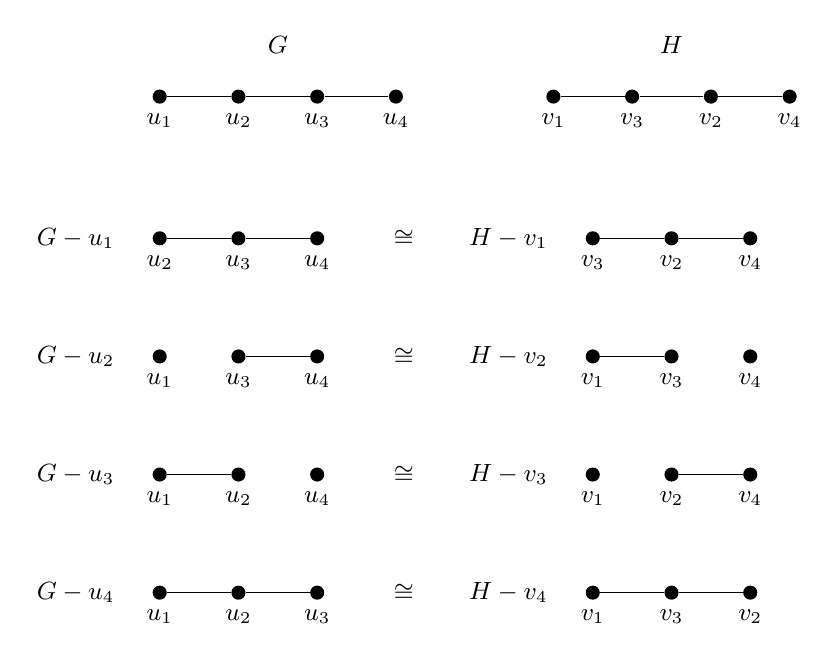
\begin{tikzpicture}[
    vertex/.style={circle, fill=black, inner sep=1.8pt},
    every label/.style={font=\small},
    graph label/.style={font=\small}
]
    % 原圖 G 與 H
    \node[graph label] at (1.5,0.65) {$G$};
    \foreach \x/\name in {0/u_1,1/u_2,2/u_3,3/u_4}
        \node[vertex, label=below:{$\name$}] (g-\name) at (\x,0) {};
    \draw (g-u_1)--(g-u_2)--(g-u_3)--(g-u_4);

    \node[graph label] at (6.5,0.65) {$H$};
    \foreach \x/\name in {5/v_1,6/v_3,7/v_2,8/v_4}
        \node[vertex, label=below:{$\name$}] (h-\name) at (\x,0) {};
    \draw (h-v_1)--(h-v_3)--(h-v_2)--(h-v_4);

    % G-u_1 與 H-v_1
    \node[graph label, anchor=east] at (-0.45,-1.8) {$G-u_1$};
    \foreach \x/\name in {0/u_2,1/u_3,2/u_4}
        \node[vertex, label=below:{$\name$}] (gu1-\name) at (\x,-1.8) {};
    \draw (gu1-u_2)--(gu1-u_3)--(gu1-u_4);
    \node[graph label] at (3.1,-1.8) {$\cong$};
    \node[graph label, anchor=east] at (5.05,-1.8) {$H-v_1$};
    \foreach \x/\name in {5.5/v_3,6.5/v_2,7.5/v_4}
        \node[vertex, label=below:{$\name$}] (hv1-\name) at (\x,-1.8) {};
    \draw (hv1-v_3)--(hv1-v_2)--(hv1-v_4);

    % G-u_2 與 H-v_2
    \node[graph label, anchor=east] at (-0.45,-3.3) {$G-u_2$};
    \node[vertex, label=below:{$u_1$}] (gu2-u1) at (0,-3.3) {};
    \node[vertex, label=below:{$u_3$}] (gu2-u3) at (1,-3.3) {};
    \node[vertex, label=below:{$u_4$}] (gu2-u4) at (2,-3.3) {};
    \draw (gu2-u3)--(gu2-u4);
    \node[graph label] at (3.1,-3.3) {$\cong$};
    \node[graph label, anchor=east] at (5.05,-3.3) {$H-v_2$};
    \node[vertex, label=below:{$v_1$}] (hv2-v1) at (5.5,-3.3) {};
    \node[vertex, label=below:{$v_3$}] (hv2-v3) at (6.5,-3.3) {};
    \node[vertex, label=below:{$v_4$}] (hv2-v4) at (7.5,-3.3) {};
    \draw (hv2-v1)--(hv2-v3);

    % G-u_3 與 H-v_3
    \node[graph label, anchor=east] at (-0.45,-4.8) {$G-u_3$};
    \node[vertex, label=below:{$u_1$}] (gu3-u1) at (0,-4.8) {};
    \node[vertex, label=below:{$u_2$}] (gu3-u2) at (1,-4.8) {};
    \node[vertex, label=below:{$u_4$}] (gu3-u4) at (2,-4.8) {};
    \draw (gu3-u1)--(gu3-u2);
    \node[graph label] at (3.1,-4.8) {$\cong$};
    \node[graph label, anchor=east] at (5.05,-4.8) {$H-v_3$};
    \node[vertex, label=below:{$v_1$}] (hv3-v1) at (5.5,-4.8) {};
    \node[vertex, label=below:{$v_2$}] (hv3-v2) at (6.5,-4.8) {};
    \node[vertex, label=below:{$v_4$}] (hv3-v4) at (7.5,-4.8) {};
    \draw (hv3-v2)--(hv3-v4);

    % G-u_4 與 H-v_4
    \node[graph label, anchor=east] at (-0.45,-6.3) {$G-u_4$};
    \foreach \x/\name in {0/u_1,1/u_2,2/u_3}
        \node[vertex, label=below:{$\name$}] (gu4-\name) at (\x,-6.3) {};
    \draw (gu4-u_1)--(gu4-u_2)--(gu4-u_3);
    \node[graph label] at (3.1,-6.3) {$\cong$};
    \node[graph label, anchor=east] at (5.05,-6.3) {$H-v_4$};
    \foreach \x/\name in {5.5/v_1,6.5/v_3,7.5/v_2}
        \node[vertex, label=below:{$\name$}] (hv4-\name) at (\x,-6.3) {};
    \draw (hv4-v_1)--(hv4-v_3)--(hv4-v_2);
\end{tikzpicture}
\end{center}

雖然對於 \(1 \le i \le 4\) 他們同構，但不是由點 \(u_i\) 對應到點 \(v_i\) 得到。

\section{路徑與連通}

\chapter{完美圖}
\section{Shannon 零錯容量}
\source{p.260}
這裡採用Fekete's lemma 去證明 \(\Psi (P) = \lim_{n \to \infty} N(n, P)^{\frac{1}{n}} \) 存在： 
\begin{lemma}[Fekete's lemma]
    If $f: \mathbb{R} \to \mathbb{R}$ satisfies that $\forall m, n \in \mathbb{N}$, $f(m+n) \le f(m) + f(n)$, then 
\[\lim_{n \to \infty} \frac{f(n)}{n}\]exists and 
\[
    \lim_{n \to \infty} \frac{f(n)}{n} = \inf _{n \ge 1} \frac{f(n)}{n}. 
\]
\end{lemma}

\begin{proof}
    Let 
    \[
        \alpha \coloneqq \inf _{n \ge 1} \frac{f(n)}{n}.
    \]
    Note that \(\alpha \) must exist since \(f(n) \ge 1\), and thus \(\frac{f(n)}{n} \ge \frac{1}{n} > 0\), which shows \(\left\{ \frac{f(n)}{n} \right\} \) is lower-bounded. 
    
    Now since for every \(n \in \mathbb{N} \) we have \(\frac{f(n)}{n} \ge \alpha\), we have 
    \[
        \liminf_{n \to \infty} \frac{f(n)}{n} \ge \alpha.
    \]  

    It suffices to show that 
    \[
        \limsup_{n \to \infty} \frac{f(n)}{n} \le \alpha. 
    \]
    Let \(\varepsilon > 0\), \(\exists k \in \mathbb{N}\) s.t. 
    \[
        \frac{f(k)}{k} < \alpha + \varepsilon.
    \]  
    Now for every sufficiently large integer \(n\), we write \(n = qk + r\), where \(0 \le r \le k - 1\). Then, by sub-additivity,
    \[
        \frac{f(n)}{n} \le q \frac{f(k)}{n} + \frac{f(r)}{n}.
    \]
    We let 
    \[
        M \coloneqq \max _{0 \le r \le k - 1} f(r),
    \]  
    then 
    \[
        \frac{f(n)}{n} \le \frac{q f(k)}{n} + \frac{M}{n}.
    \]
    Now \(q = \frac{n - r}{k}\), we have 
    \[
        \frac{f(n)}{n} \le \frac{n - r}{k} \frac{f(k)}{n} + \frac{M}{n} = \frac{n - r}{n} \frac{f(k)}{k} + \frac{M}{n} \le \frac{f(k)}{k} + \frac{M}{n} < \alpha + \varepsilon + \frac{M}{n}.
    \] 
    Taking limsup on both sides, we have 
    \[
        \limsup_{n \to \infty} \frac{f(n)}{n} \le \limsup_{n \to \infty} \alpha + \varepsilon + \frac{M}{n} = \alpha + \varepsilon.  
    \]
    Since this is true for all \(\varepsilon > 0\), we have 
    \[
        \limsup_{n \to \infty} \frac{f(n)}{n} \le \alpha, 
    \] 
    and thus now we have 
    \[
        \alpha \le \liminf_{n \to \infty} \frac{f(n)}{n} \le \limsup_{n \to \infty} \frac{f(n)}{n} \le \alpha. 
    \]
    This shows 
    \[
        \lim_{n \to \infty} \frac{f(n)}{n} = \alpha = \inf _{n \ge 1} \frac{f(n)}{n}. 
    \]
\end{proof}

Now we can show \(\Psi (P) = \lim_{n \to \infty} N(n, P)^{\frac{1}{n}} \) exists by applying Fekete's lemma.

\begin{proof}
    Suppose \(f(n) = -\log N(n, p)\), then for any \(m, n \in \mathbb{N}\) we have
    \begin{align*}
        f(m + n) &= -\log N(m + n, P) \le - \log (N(m, P) N(n, P)) \\
        &= -\log N(m, P) - \log N(n, P) = f(m) + f(n).
    \end{align*} 
    Therefore, by Fekete's lemma, 
    \[
        \lim_{n \to \infty} \frac{f(n)}{n}
    \]
    exists, which means 
    \[
        \lim_{n \to \infty} -\frac{1}{n} \log N(n, P)
    \]
    exists, and since \(f(x) = e^x\) is continuous, 
    \[
        \lim_{n \to \infty} N(n, p)^{\frac{1}{n}} = \lim_{n \to \infty} e^{\frac{1}{n} \log N(n, P)} 
    \] 
    should also exist.
\end{proof}